% Diagrama de conexión entre el ESP32 y la cámara OV2640 (placa ESP32-CAM).
% Se compila por separado: pdflatex conexion_camara.tex -> conexion_camara.pdf
\documentclass[tikz,border=4pt]{standalone}
\usepackage[utf8]{inputenc}
\usepackage[T1]{fontenc}
\usepackage{cmbright}
\usetikzlibrary{arrows.meta}

% Mismos colores que el diagrama de la ONX3248G035
\definecolor{ci2s}{RGB}{31,94,168}
\definecolor{ci2c}{RGB}{190,100,10}
\definecolor{cpwm}{RGB}{130,50,140}
\definecolor{cdir}{RGB}{90,90,90}

\begin{document}
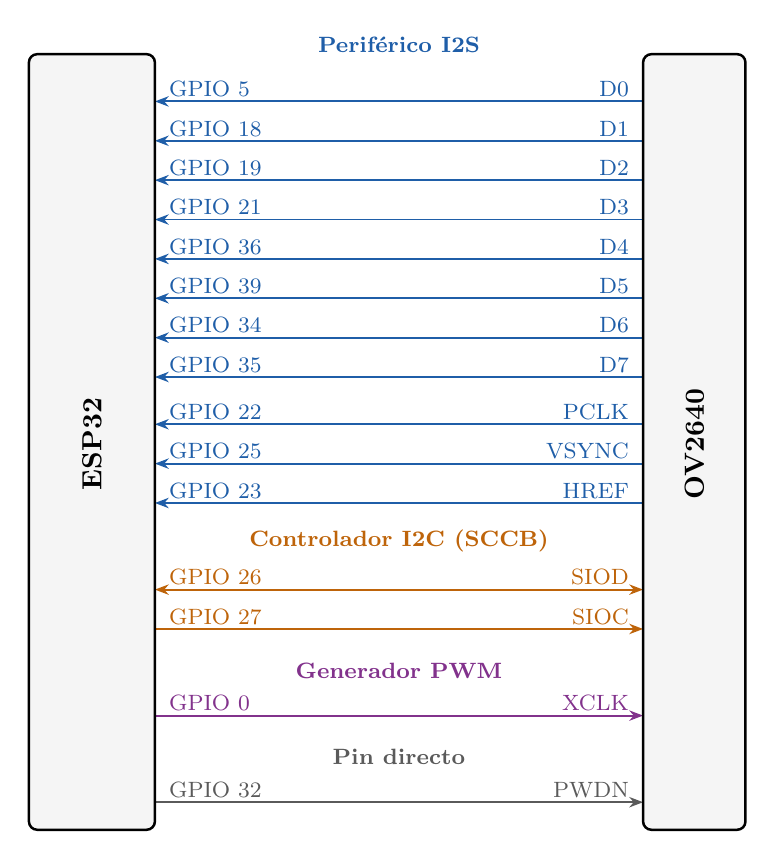
\begin{tikzpicture}[
    font=\small,
    senal/.style={line width=0.7pt},
    caja/.style={draw, line width=0.9pt, rounded corners=3pt, fill=gray!8},
    gpio/.style={anchor=south west, font=\footnotesize, inner sep=1.5pt},
    nombre/.style={anchor=south east, font=\footnotesize, inner sep=1.5pt},
    grupo/.style={font=\footnotesize\bfseries, anchor=south},
    >={Stealth[length=5pt]}
]
\def\xa{0}      % borde derecho del ESP32
\def\xb{6.2}    % borde izquierdo de la OV2640
\def\xg{3.1}    % posición de los rótulos de grupo

% ---------------- Periférico I2S: datos y sincronización ----------------
\node[grupo, ci2s] at (\xg,0.25) {Periférico I2S};
\foreach \n/\g/\y in {
    D0/5/-0.25, D1/18/-0.75, D2/19/-1.25, D3/21/-1.75,
    D4/36/-2.25, D5/39/-2.75, D6/34/-3.25, D7/35/-3.75,
    PCLK/22/-4.35, VSYNC/25/-4.85, HREF/23/-5.35} {
    \draw[senal, ci2s, <-] (\xa,\y) -- (\xb,\y);
    \node[gpio, ci2s] at (\xa+0.12,\y) {GPIO \g};
    \node[nombre, ci2s] at (\xb-0.12,\y) {\n};
}

% ---------------- Controlador I2C: bus SCCB ----------------
\node[grupo, ci2c] at (\xg,-6.1) {Controlador I2C (SCCB)};
\draw[senal, ci2c, <->] (\xa,-6.45) -- (\xb,-6.45);
\draw[senal, ci2c, ->]  (\xa,-6.95) -- (\xb,-6.95);
\node[gpio, ci2c] at (\xa+0.12,-6.45) {GPIO 26};
\node[gpio, ci2c] at (\xa+0.12,-6.95) {GPIO 27};
\node[nombre, ci2c] at (\xb-0.12,-6.45) {SIOD};
\node[nombre, ci2c] at (\xb-0.12,-6.95) {SIOC};

% ---------------- Generador PWM: reloj de la cámara ----------------
\node[grupo, cpwm] at (\xg,-7.7) {Generador PWM};
\draw[senal, cpwm, ->] (\xa,-8.05) -- (\xb,-8.05);
\node[gpio, cpwm] at (\xa+0.12,-8.05) {GPIO 0};
\node[nombre, cpwm] at (\xb-0.12,-8.05) {XCLK};

% ---------------- Pin directo: apagado ----------------
\node[grupo, cdir] at (\xg,-8.8) {Pin directo};
\draw[senal, cdir, ->] (\xa,-9.15) -- (\xb,-9.15);
\node[gpio, cdir] at (\xa+0.12,-9.15) {GPIO 32};
\node[nombre, cdir] at (\xb-0.12,-9.15) {PWDN};

% ---------------- Bloques ----------------
\draw[caja] (\xa-1.6,0.35) rectangle (\xa,-9.5);
\node[rotate=90, font=\bfseries] at (\xa-0.8,-4.6) {ESP32};
\draw[caja] (\xb,0.35) rectangle (\xb+1.3,-9.5);
\node[rotate=90, font=\bfseries] at (\xb+0.65,-4.6) {OV2640};
\end{tikzpicture}
\end{document}
